\documentclass[journal]{IEEEtran}
\usepackage{amsmath}
\usepackage{graphicx}
\usepackage{tikz}
\usepackage{color}
\usetikzlibrary{shapes,arrows}
\usepackage{subcaption}
\newcommand\blfootnote[1]{%
  \begingroup
  \renewcommand\thefootnote{}\footnote{#1}%
  \addtocounter{footnote}{-1}%
  \endgroup
}

\newcommand{\ab}[1]{\textcolor{red}{#1}}
\newcommand{\vj}[1]{\textcolor{blue}{#1}}

\usepackage[style=ieee,backend=bibtex, maxbibnames=5]{biblatex}
\bibliography{library.bib}
\title{MOABB: Trustworthy algorithm benchmarking for BCIs}
\author{
  \IEEEauthorblockN
  {
    Vinay Jayaram\IEEEauthorrefmark{1}\IEEEauthorrefmark{2},
    Alexandre Barachant\IEEEauthorrefmark{3}
  }

  \IEEEauthorblockA
  {
    \IEEEauthorrefmark{1}
    Max Planck Institute for Intelligent Systems, 
    Department Empirical Inference, 
    T\"{u}bingen, Germany \\
    Email: vjayaram@tue.mpg.de}
  
  \IEEEauthorblockA
  {
    \IEEEauthorrefmark{2}
    IMPRS for Cognitive and Systems Neuroscience, 
    University of T\"{u}bingen, 
    T\"{u}bingen, Germany \\
  }
  \IEEEauthorblockA
  {
    \IEEEauthorrefmark{3}
    CTRL-Labs,
    New-York, USA \\
    Email: alexandre.barachant@gmail.com
  }
}
\begin{document}
\maketitle
\begin{abstract}
  BCI algorithm development has long been hampered by two major issues: Small
sample sets and a lack of reproducibility. We offer a solution to both of these
problems in the form of a software suite that simplifies and streamlines both
the issue of finding, downloading, and preprocessing data in a reliable manner,
and the issue of a reliable interface to use machine learning methods. By
building on recent advances in software for signal analysis implemented in the MNE toolkit,
and the unified framework for machine learning offered by the scikit-learn
project, we offer a system that can improve BCI algorithm development. To
validate this system, we analyze of a set of state-of-the-art decoding
algorithms across many open access datasets. Our analysis confirms that
different datasets can result in very different results for identical processing
pipelines, highlighting the need for a trustworthy algorithm benchmarking in the
field of BCIs., and further that many previously validated results do not hold
up when applied across different datasets, which has wide-reaching implications
for practical BCIs.

%%% Local Variables:
%%% mode: latex
%%% TeX-master: "main"
%%% End:

\end{abstract}
\section{Introduction}
Brain-computer interfaces (BCIs) have long presented the neuroscience methods
community with a unique challenge. Unlike fields like vision research, where one
simply has a database of images and labels, a BCI is defined by a signal
recorded from the brain and fed into a computer, which can be influenced in any
number of ways both by the subject and by the experimenter. As a result,
validating approaches has always been a difficult task. Number of channels,
requested task, physical setup, and many other features vary between the
numerous publically available datasets online, not to mention issues of
convenience such as file format and documentation. Because of this, the BCI
methods community has long done one of two things to validate an new approach:
Recorded a new dataset, or used one of few well-known, tried-and-true datasets.

Recording a new dataset, though an elegant way to show that a proposed
method works online, presents problems for post-hoc analysis. Without
making data public, it is impossible to know whether offline
classification results are convincing or due to some coding issue or
recording artifact. Further, it is well-known that differences in
hardware \cite{Searle2000,Lopez-Gordo2014}, paradigm \cite{Allison2010}, and
subject \cite{Allison2010} can have large differences in the
outcome of a BCI task, making it very difficult to generalize findings
from any single dataset.

When recording a new dataset is not an option, One can turn to some of
the standard EEG datasets publicly available. Over the course of the
last year and a half, over a thousand journal and conference
submissions have been written on the BCI Competition III
\cite{Blankertz2006,Schloegl2005} and IV \cite{Tangermann2012}
datasets. Considering that these datasets have been available
publically for over a decade, the true number of papers which validate
results against them is simply astronomical. While it is impossible to
argue about the impact those two datasets have had on the field,
relying so heavily on a small number of datasets, with less than 50
subjects total, expose the field to several important issues. In
particular, overfitting to the setups offered there is likely.

Lastly, and possibly most problematically, the scarcity of available
code for newly published BCI algorithm puts the onus on each
individual lab to reproduce the code for all other competing methods
in order to make a claim to be comparable with the 'state-of-the-art'
(SOA). As a result, the vast majority of novel BCI algorithm papers
compare either against other work from the same lab, or old standards
such as CSP \cite{Koles1990},
with or without regularization, and LDA, or simple channel-level
variances combined with a classifier of choice \cite{Garrett2003} .

Computer vision has solved this problem with enormous datasets like
\cite{Deng2009} bundled with a reliance on a small number of software
packages to create new models, notably Tensorflow, Theano, and
Pytorch. As BCIs are inextricably linked to human use, it is not
helpful to create datasets of such size. Rather, the field requires
as many unique people recording data in many contexts in order to
create an appropriate benchmark. In contrast to image data, the goal
of BCI algorithm development is exclusively to create algorithms that
work on data that has not yet been recorded. We propose our platform, the MOABB
(Mother Of All BCI Benchmarks) Project, as a candidate for this application. 

As an initial validation of this project, we present results on the
constrained task of binary classification in two-class imagined motor
imagery, as that is the most widely used motor imagery paradigm and
allows us to demonstrate the process across the largest number of
datasets.  However, we note that this is only the first question we
attempt to answer in this field. The format allows for many other questions,
including different channel types (EEG, fNIRS, or other), multi-class
paradigms, and also transfer learning scenarios as described in
\cite{Jayaram2016}. \vj{...yeah it's a bit gratuitous. Too much?}

%%% Local Variables:
%%% mode: latex
%%% TeX-master: "main"
%%% End:

\section{Methods}
Any BCI analysis is defined by three things: A dataset, a context, and
a processing pipeline. Here we describe how all of these components
are dealt with within our pipeline, and how specifically we set the
options for the initial analyses presented here.

\subsection{Datasets}

Public BCI datasets exist for a wide range of user paradigms and
recording conditions, from continuous usage to single-session to
multiple-sessions-per-subject. Within the current MOABB project, we
have unified the access to many datasets, described in Table
\ref{fig:datasets}.


\begin{table*}[ht]
  \centering
  \begin{tabular}{l || c | c | c | c | c | c | c }
    Name & Imagery & \# Channels & Avg \# Trials & \# Sessions & \# Subjects & Epoch & Citations \\ \hline
    Cho et al. 2017 & Right, left hand & 64 & 200 & 1 & 49 & 0-3s & \cite{Cho2017} \\
    Physionet & Right, left hand & 64 & 45 & 1 & 109 & 1-3s & \cite{Schalk2004, Goldberger2000} \\
    Shin et al. 2017 & Right, left hand & 25 & 60 & 1 & 29 & 0-10s & \cite{Blankertz2007, Shin2017} \\
    BNCI 2014-001 & Right, left hand & 22 & 288 & 2 & 9 & 2-6s & \cite{Tangermann2012} \\
    BNCI 2014-002 & Right hand, feet & 15 & 160 & 1 & 14 & 3-8s & \cite{Steyrl2016a} \\
    BNCI 2014-004 & Right, left hand & 3 & 720 & 2 & 9 & 3-7.5s & \cite{Leeb2007} \\
    BNCI 2015-001 & Right hand, feet & 13 & 400 & 2 & 13 & 3-8s & \cite{Faller2012} \\
    BNCI 2015-004 & Right hand, feet & 30 & 155 & 2 & 10 & 3-10s & \cite{Scherer2015} \\
    Alexandre Motor Imagery & Right hand, feet & 16 & 40 & 1 & 9 & 0-3s & \cite{Barachant2012a}\\
    Yi et al. 2014 & Right, left hand & 60 & 160 & 1 & 10 & 3-7s & \cite{Yi2014} \\
    Zhou et al. 2016 & Right, left hand & 14 & 100 & 3 & 4 & 1-6s & \cite{Zhou2016a}\\
    
\end{tabular}
    \caption{Dataset attributes}
    \label{fig:datasets}
\end{table*}

Adding new datasets that can be found on the internet is also
simple. The MNE toolkit \cite{Gramfort2014,Gramfort2013} is used for
all preprocessing and channel selection, so any dataset that can be
made compatible with their framework can quickly be added to the set
of data offered by this project. In addition, the project offers test
functions to ensure candidate code conforms to the software interface.

\subsection{Context}

A \emph{context} is the set of characteristics that defines the
preprocessing and validation procedure. To go from a recorded EEG
time-series to a pipeline performance value for a given subject or
recording session, many parameters must be defined. First, trials need to be
cut out of the continuous signal and pre-processed, which is
possible in many different ways when taking into account parameters such as
trial overlap, trial length, imagery type, and more. Once the
continuous data is processed into trials, and these trials are fed
into a pipeline, the next question of how to create training and test sets,
and how to report performance, comes into play. We separate these two
notions in our software and call them the \emph{paradigm} and the
\emph{evaluation} respectively.

\subsubsection{Paradigm}

A paradigm defines how one goes from continuous data to trials for a
standard machine learning pipeline to deal with. While not an issue
in image processing, it is crucial in EEG and biosignals processing
because most datasets do not have exactly the same events defined in
the continuous data. For example, many datasets with two-class motor imagery use left versus right hand, while some use hands versus feet; 
there are also many possible non-motor imageries. For any reasonable
analysis the specific sort of imagery or ERP must be controlled for,
as they all have different characteristics in the data and further are
variably effective across subjects \cite{Scherer2015,Allison2010}. After choosing
which events or imageries are valid, the question comes to
pre-processing of the continuous data, in the form of ICA cleaning,
bandpass filtering, and so on. These must also be identical for valid
comparisons across algorithm or datasets. Lastly, there are questions
of how to cut the data into trials: What is the trial length and
overlap; or, in the case of ERP paradigms, how long before and after
the event marker do we use? The answers to all these questions are
summed up in the paradigm object.

\subsubsection{Evaluation}

Once the data is split into trials and a pipeline is fixed, there are many ways
to train and test this pipeline to minimize overfitting. For datasets with
multiple subjects recorded on multiple days, we may want to determine which
algorithm functions best in multi-day classification. Or, we may want to
determine which algorithm is best for small amounts of training data. It is easy
to see that there are many possibilities for splitting data into train and test
sets depending on the question to be answered, and these must be fixed
identically for a given analysis. Furthermore, there is the question of how to
report results. Multiclass problems cannot use metrics like the ROC-AUC which
provide unbiased estimates of classifier goodness in binary cases; depending on
things like the class balance, various other metrics have their own benefits and
pitfalls. Therefore this must also be fixed across all datasets, contingent on
the class of predictions the pipelines attempt to make. We define this as our
\emph{evaluation}.

\subsection{Pipeline}

We define a \emph{pipeline} as the processing that takes one from raw
trial-wise data into labels, taking both spatial filtering and
classification model fitting into account. A convenient API for
dealing with this kind of processing is defined by
scikit-learn \cite{Pedregosa2011}, which allows for easily definable
dimensionality reduction, feature generation, and model fitting. To
maximize reproducibility we allow pipelines to be defined either by
yaml files or through python files that generate the objects, but
force all machine learning models to follow the scikit-learn
interface. 

\section{Statistical Analysis}
\label{stats}

At the end of processing there are scores for every subject in every
dataset with every pipeline. The goal of this project is to synthesize
these numbers into an estimate of how likely it is that each pipeline
out-performs the other pipelines. However, even if imagery type and
channel number were held constant, differences in trial amount,
sampling rate, and even location and hardware mean that we cannot
expect subjects across datasets to be naively comparable. Simply
pooling them all and running a paired-sample test would result in
misleading significances due to these factors. This would
suggest a mixed-factor ANOVA for every unique pair of pipelines to
test the null hypothesis that the difference distribution is zero-mean
over all datasets. However, we have the secondary problem that this
difference distribution, even within a given dataset, is very unlikely
to be Gaussian (which is an assumption of an ANOVA). It is well-known
that some subjects are BCI illiterate, which implies that no pipeline
can reliably out-predict another one on that subset of
subjects. Therefore, for large enough datasets, the distribution of
differences in pipeline scores is very likely to be at least bimodal.

Thankfully, a similar statistical situation has already arisen in the
field of medical studies. It is often the case that one wants to
measure a quantity from multiple groups of subjects (different
hospitals, for examples) at multiple time points, then ask if there
was a significant effect of time in the measurements. This type of
study design is called a \emph{factorial design} and is equivalent to
the design described above (where instead of time we have different
pipelines). Restricting each test to two pipelines gives us a way of
generating a p-value for the difference between the two. To deal with
the non-Gaussianity, we use non-parametric, rank-based computation of
the test statistics as described in \cite{Noguchi2012}, and we can use
Bonferroni correction to deal with the fact that each pipeline will
appear $N_{\text{pipelines}} - 1$ times.

\section{Experiment}

To show off the possibilities of this framework, we ran various well-known BCI
pipelines from across many papers in order to conduct the first big-data,
side-by-side analysis of the state of the art in motor imagery BCIs.

\subsection{Context}
For the paradigm, we choose to look at datasets including motor
imagery.  Motor imagery is the most-studied sort of imagery for BCIs
\cite{Yuan2014}, and we further limit ourselves to the binary case as
this has not yet been solved. For evaluations, we choose
within-session cross-validation, as this represents the best-case
scenario for any pipeline, with minimal non-stationarity. 

\subsubsection{Paradigm}
As there are many methods that show that multiple frequency bands can
lead to improved BCI performance\cite{KaiKengAng2008}, and further
that discriminative data is concentrated in the anatomical frequency
bands, we test three preprocessing pipelines: A single bandpass
containing both the alpha and beta ranges, from $8-32\text{Hz}$,
another from $8-32\text{Hz}$ in 4Hz increments, and a third with the
$\delta, \theta, \alpha$ and $\beta$ frequencies isolated.

\subsubsection{Evaluation}
The evaluation was chosen to be within-session, as that minimizes the
effect of non-stationarity. As this is a binary classification task,
the ROC-AUC score was chosen as the metric to score 5-fold cross
validation (the splits were kept identical for all pipelines). In
order to return a single score per subject, the scores from each
session were averaged when multiple sessions were present.

\subsection{Pipelines}

Given the sheer breadth of models implemented within scikit-learn,
attempting an exhaustive model comparison would be impossible. Instead, we
implement a selection of pipelines from the BCI literature, as well as the
well-known standards of CSP + LDA and channel-level variances + SVM. Specific
implemented pipelines are in Table \ref{tab:pipelines}; all hyperparameters were set via cross-validation.
\begin{table*}
  \centering
  \begin{tabular}{ l || p{6cm} | p{6cm} | c | }
    
    Name & Preprocessing & Classifier \\ \hline
    CSP + LDA & Trial covariances estimated via maximum-likelihood with unregularized common spatial patterns (CSP). Features were log variance of the filters belonging to the 6 most diverging eigenvalues & Linear Discriminant Analysis (LDA) & \cite{Koles1990} \\ \hline
    RegCSP + shLDA & Trial covariances estimated by OAS (Chen) with
                     unregularized CSP. This is equivalent to Tikhonov
                     regularization as described in \cite{Lotte2011}. Features were log variance on the 6 top filters. & LDA with Ledoit-Wolf shrinkage of the covariance term  & \cite{Lotte2011} \\ \hline
    rieCSP + shLDA & Trial covariances estimated via maximum-likelihood, CSP class-wise matrices were Riemannian mean of the trial-wise matrices. & LDA with Ledoit-Wolf shrinkage of the covariance term  & \cite{TODO} \\ \hline
    FBCSP + optSVM & Filter bank of 6 bands between 8 and 35 Hz followed by OAS covariance estimation and unregularized CSP. Log variance from each of the 4 top filters from each sub-band were pooled and the top 10 features chosen by mutual information were used. & A linear support vector machine was trained with its regularization hyperparameter set by a cross-validated grid-search from $[0.01 100]$. & \cite{KaiKengAng2008} \\ \hline
    TS + optSVM & Trial covariances estimated via OAS then projected into the Riemannian tangent space to obtain features & Linear SVM with identical grid-search & \cite{Barachant2013} \\ \hline
    AM + optSVM & Log variance in each channel & Linear SVM with grid-search & N/A \\ \hline
    FB-AM + optLR & Log variance from each channel in the five anatomical frequency bands ($\delta, \theta, \alpha, \beta, \gamma$) & To replicate the genetic algorithm and channel selection used in the paper, as well as the linear final boundary, we use a logistic regression classifier with an L1 penalty, hyperparameter optimized via grid search& \cite{Garrett2003} \\
    
  \end{tabular}
  \caption{Processing pipelines}
  \label{tab:pipelines}
\end{table*}
  

%%% Local Variables:
%%% mode: latex
%%% TeX-master: "main.tex"
%%% End:

\section{Results}
The results from analyses with this data will be displayed in three plots, described below:

\subsubsection{Score plot}
The first plot displays the raw results as a violin plot per algorithm and
dataset. With a reasonably small number of datasets as we have here, the plot is
quite informative; however, as the number of datasets increases it will become
more and more dense. It describes the distribution of scores over subjects
within a single dataset and for a single algorithm. Within each dataset, as
described in \ref{stats}, an ANOVA is computed. If the p-value of the result is
low enough, the dataset is highlighted green to show that there is a significant
difference between pipelines within it.

\subsubsection{Ranking plot}
Once a difference is significant, post hoc testing is displayed in the ranking
plot. Here, the colors corresponding to the different methods are ranked as
described in \ref{stats} and for each dataset, these sets of equally-performing
algorithms are displayed. To summarize the results of the analysis, the
final plot is a bar plot that describes how many times each algorithm was in the
best-performing subset.

\subsubsection{Time plot}
(note: time plot should be over *all* analyses...)  In addition to accuracy,
model fitting time can also affect which pipeline is most appropriate for a
given situation. This is a function of both the number of channels, timepoints,
and samples, but a point cloud in three-dimensions is difficult to visualize on
paper. As such, for these written reports, a plot is generated of the time
versus the number of entries in the training matrix, which is the product of the
number of channels and the number of samples (the number of timepoints is less
important as features are usually computed over all of them). While some of the
nuance is lost, it is still easy to see how algorithms compare to each other.

\begin{figure*}
    \centering
    \begin{subfigure}[t]{\textwidth}
        \centering
        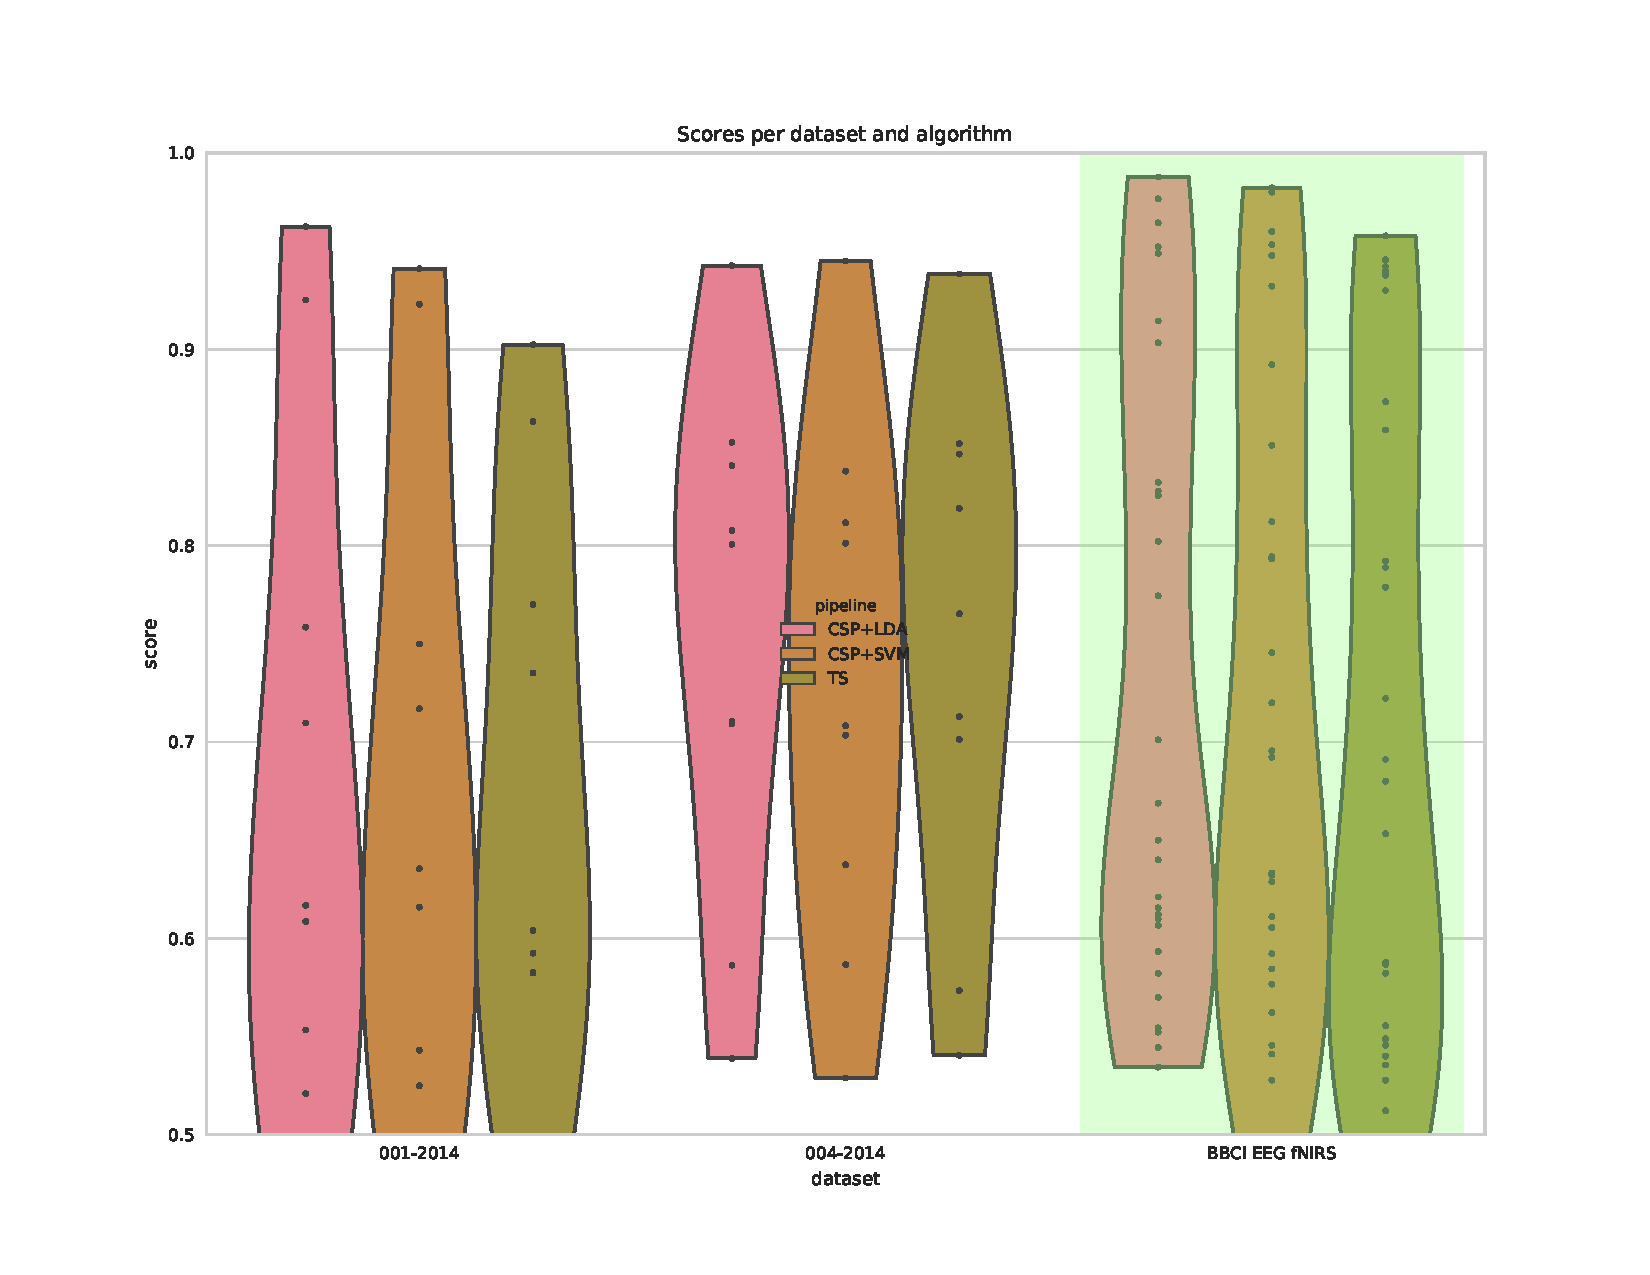
\includegraphics[width=\textwidth]{CrossSubjectEvaluation_/scores.pdf}
    \end{subfigure}%
     
    \begin{subfigure}[h]{0.45\textwidth}
        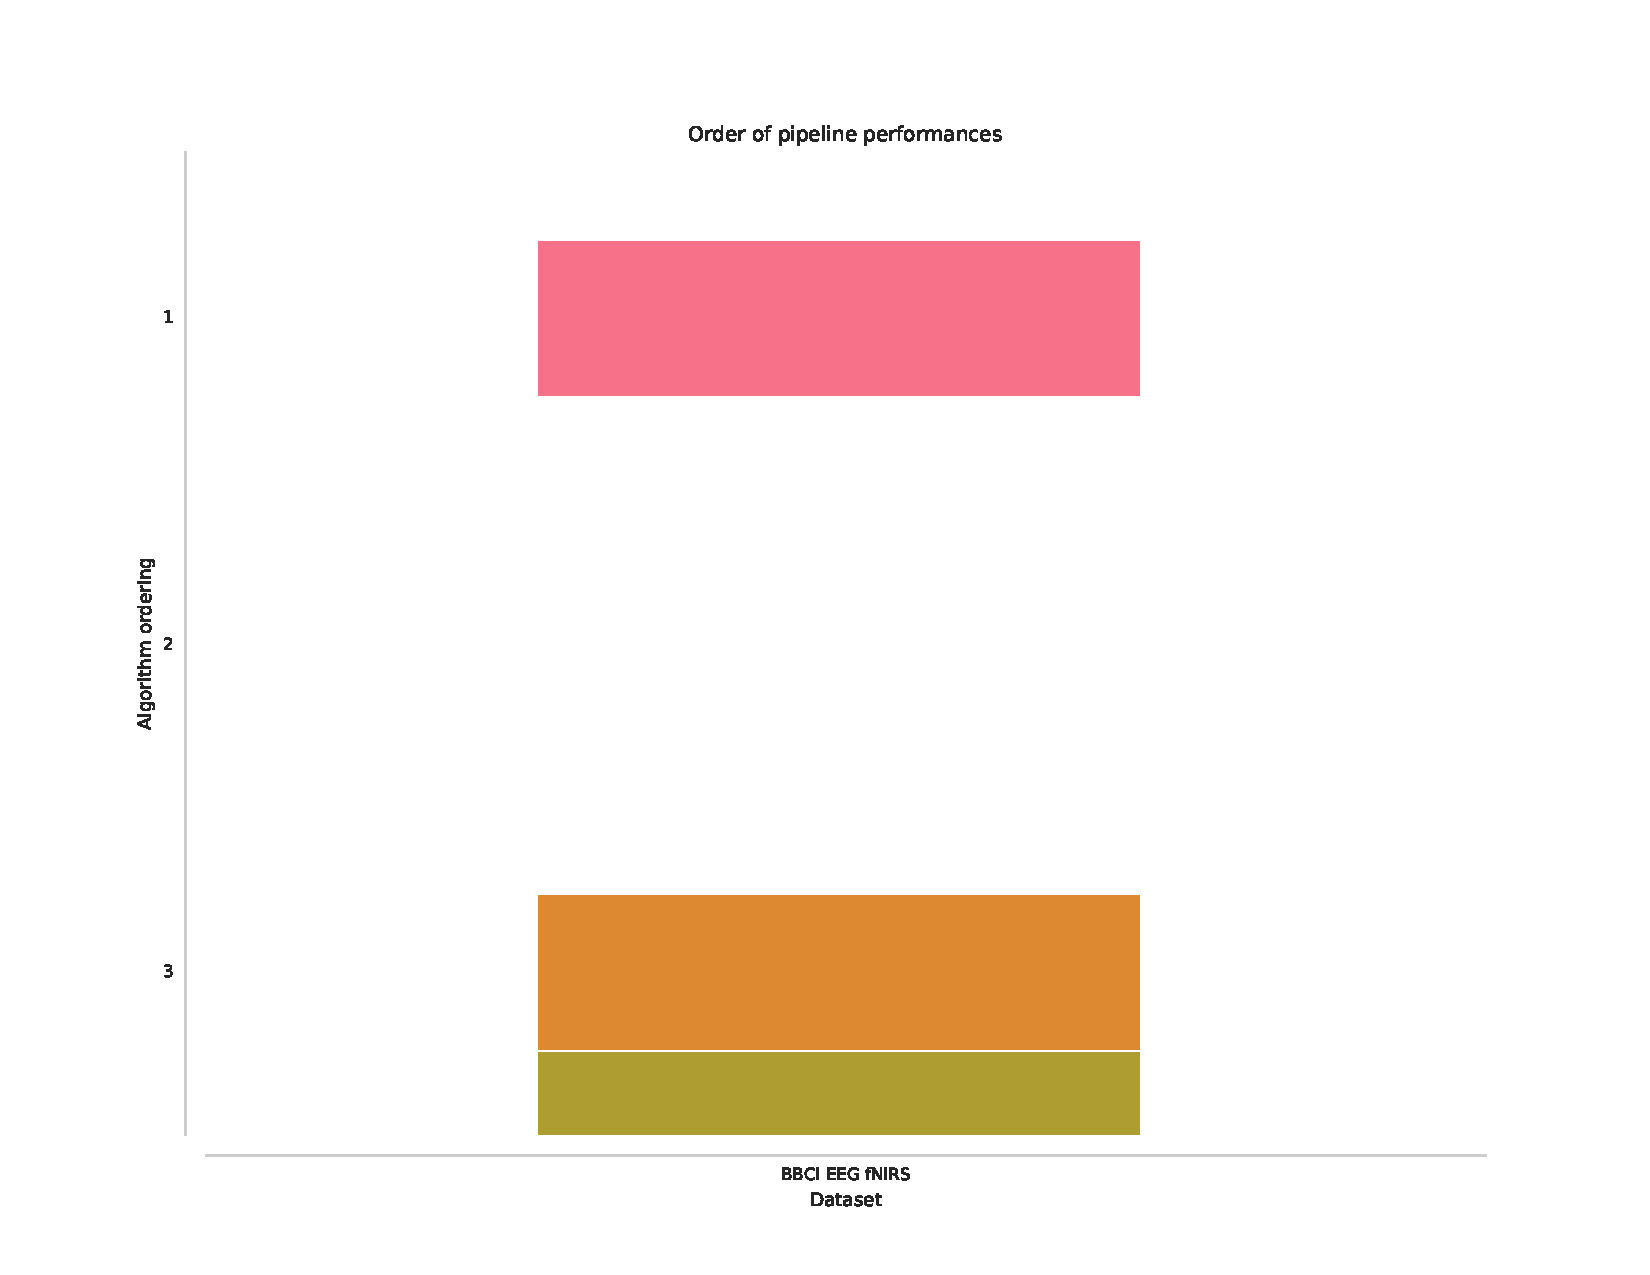
\includegraphics[width=\textwidth]{./CrossSubjectEvaluation_/ordering.pdf}
    \end{subfigure}
    \begin{subfigure}[h]{0.45\textwidth}
        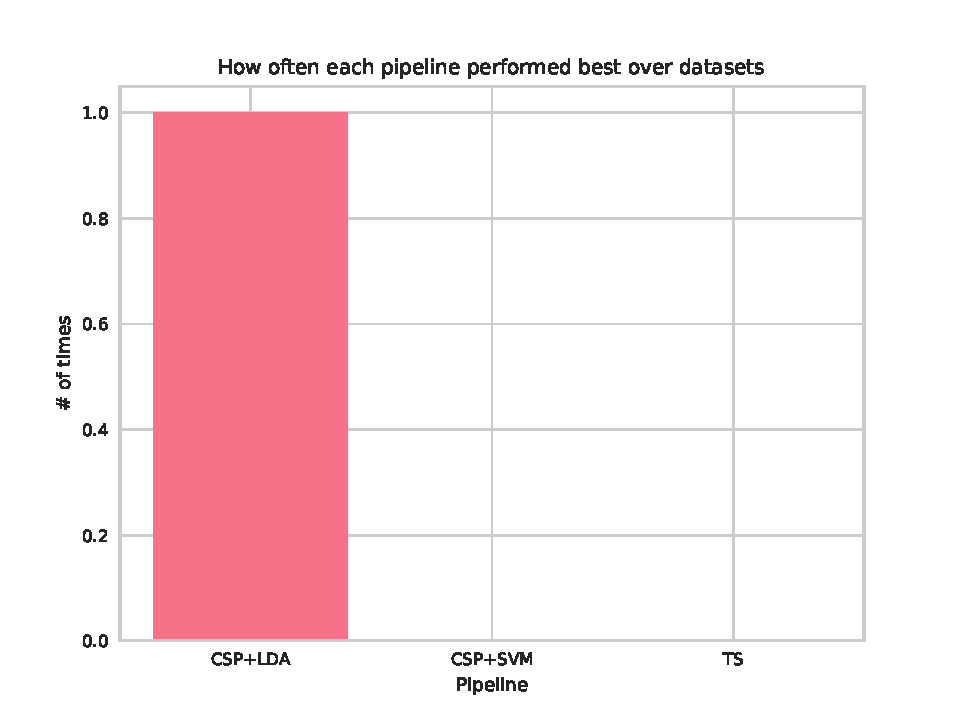
\includegraphics[width=\textwidth]{./CrossSubjectEvaluation_/summary.pdf}
    \end{subfigure}
    \caption{Cross-subject evaluation using all channels}
\end{figure*}
\begin{figure*}
    \centering
    \begin{subfigure}[t]{\textwidth}
        \centering
        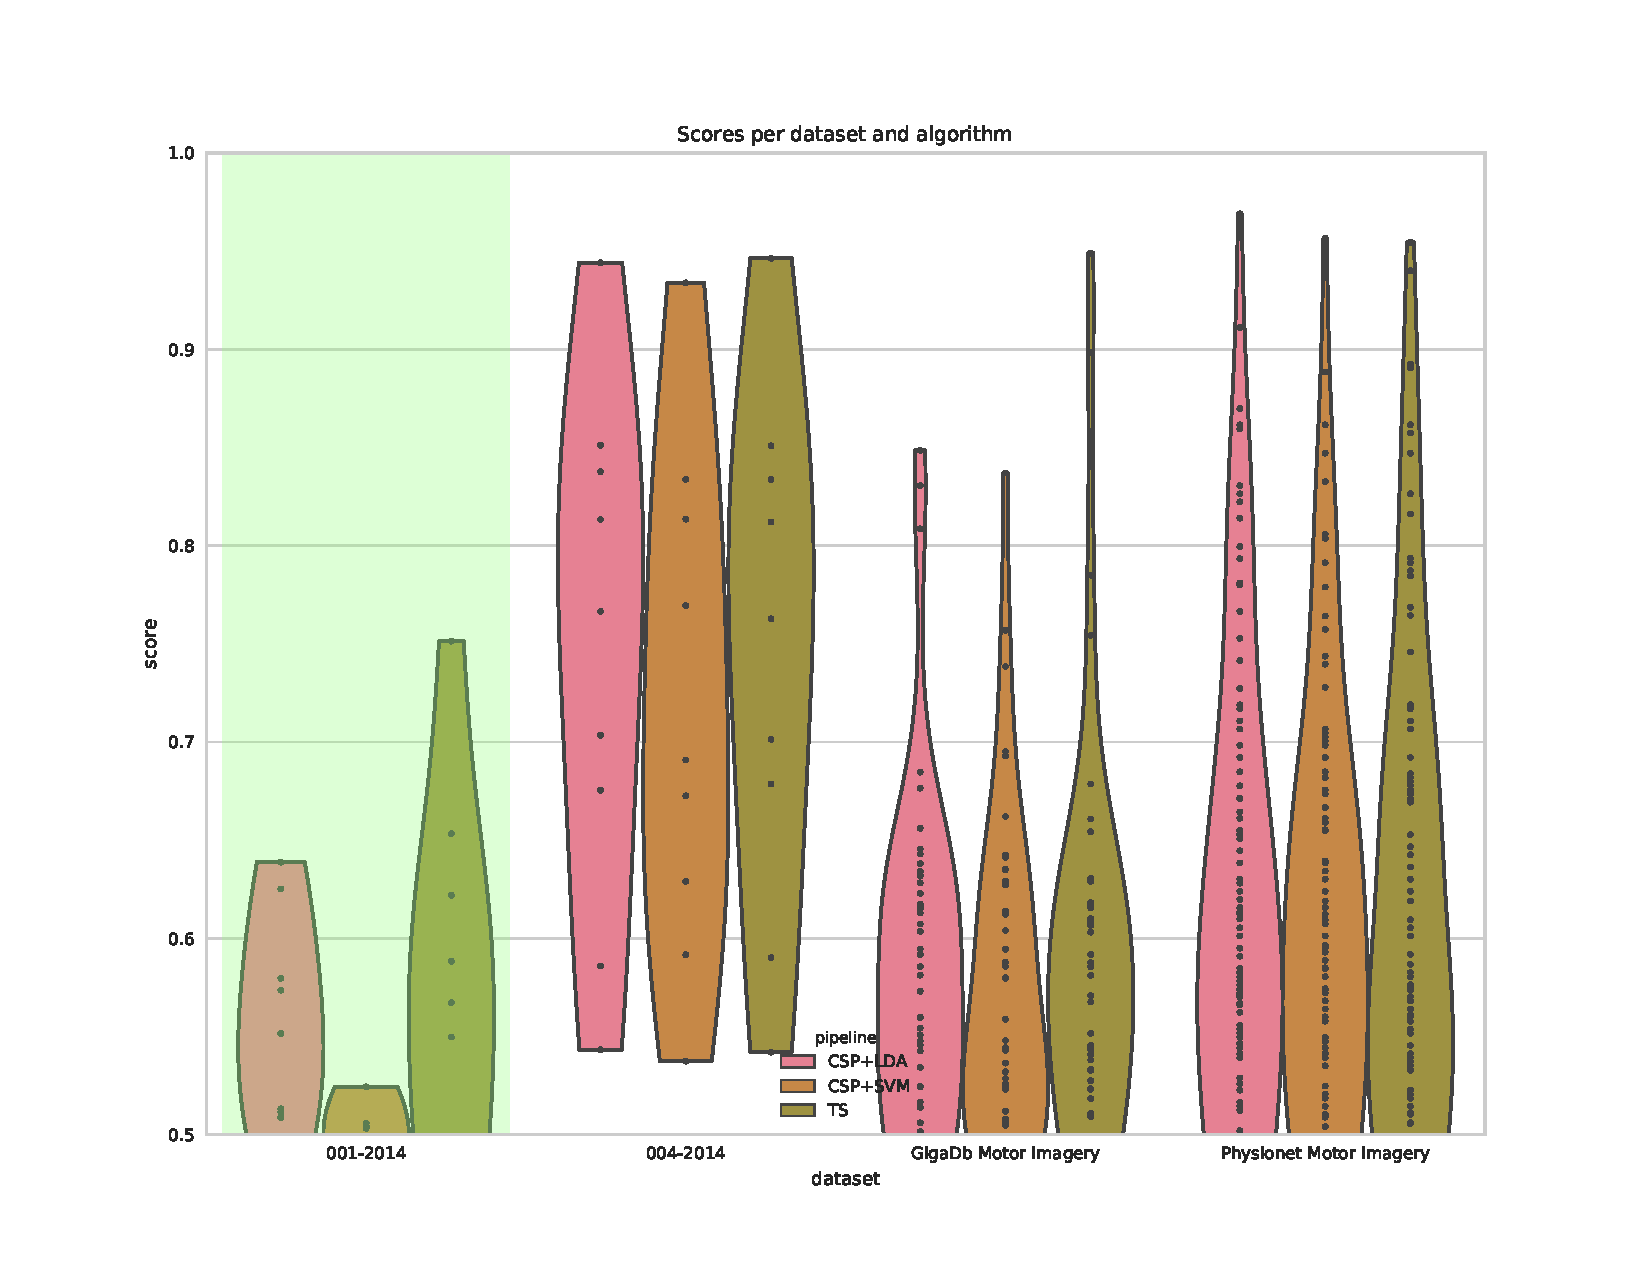
\includegraphics[width=\textwidth]{CrossSubjectEvaluation_C3C4/scores.pdf}
    \end{subfigure}%
     
    \begin{subfigure}[h]{0.45\textwidth}
        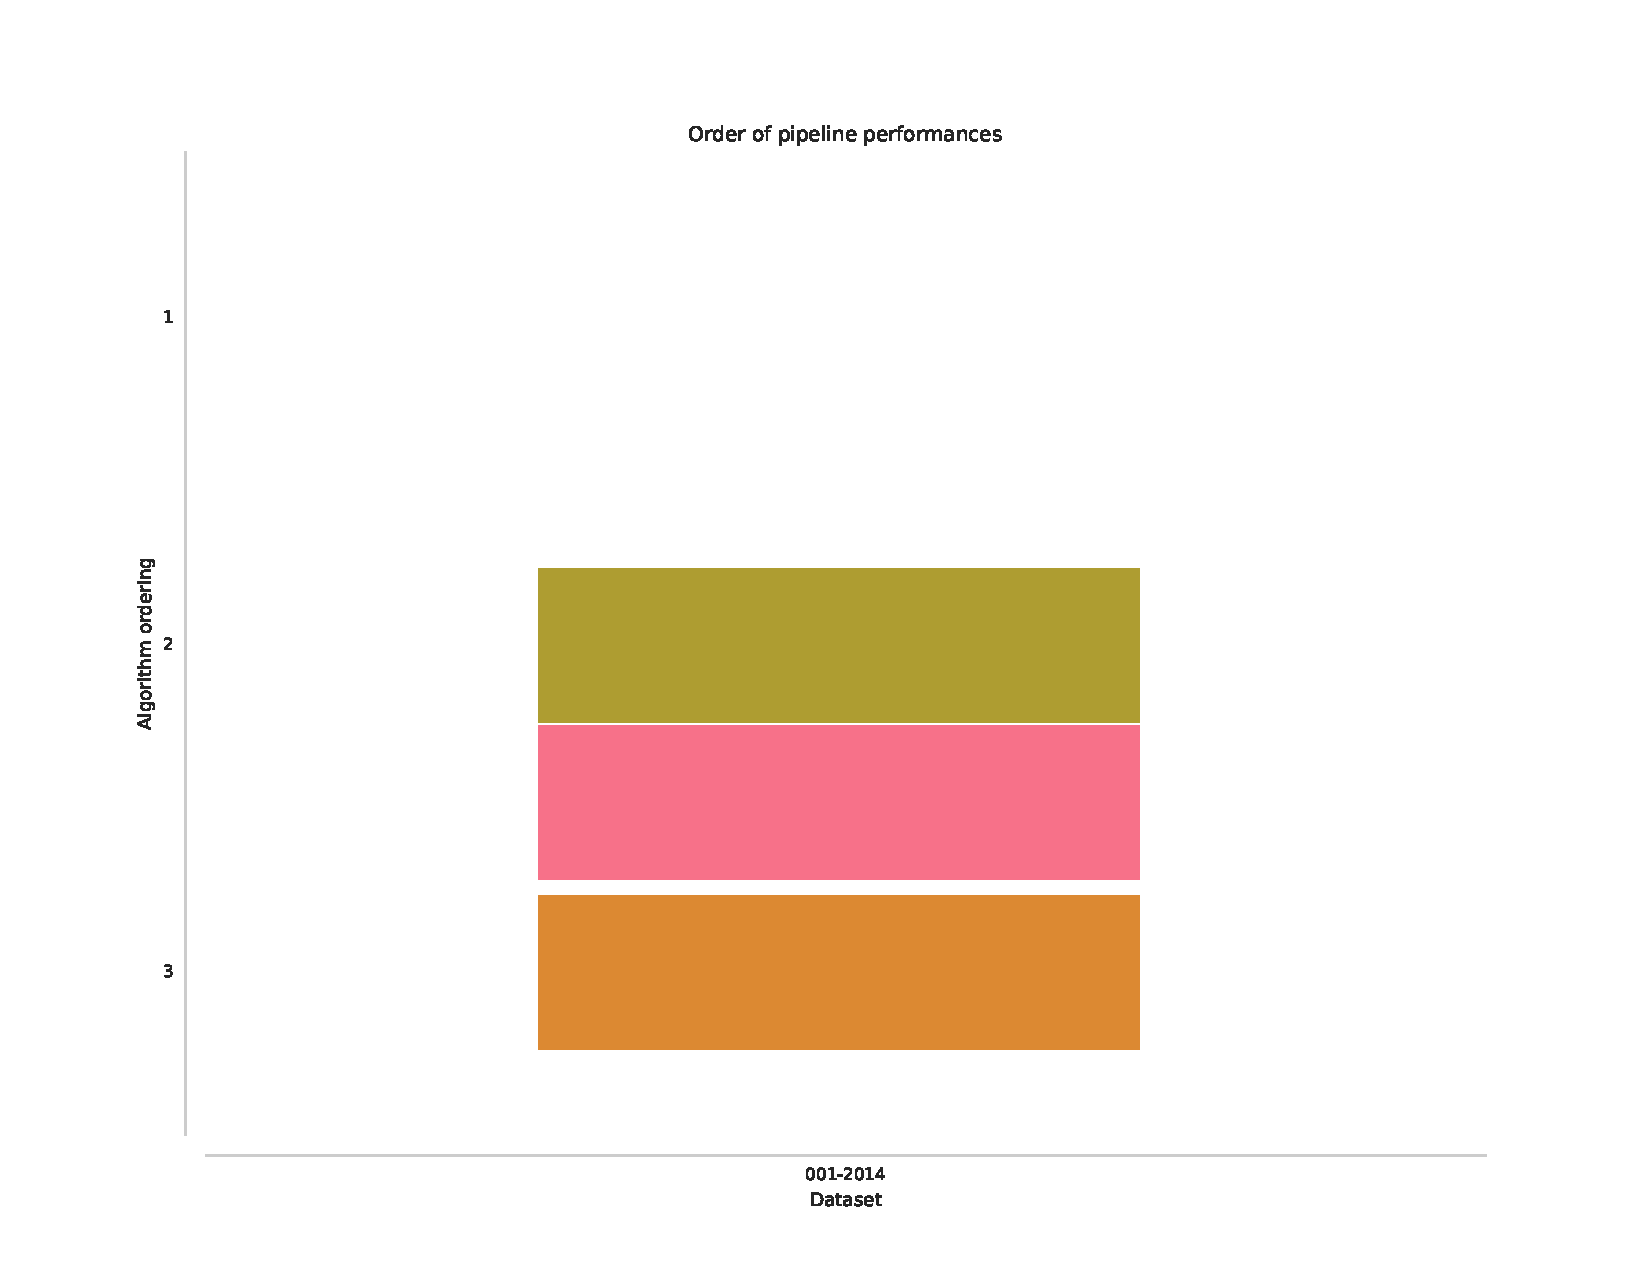
\includegraphics[width=\textwidth]{./CrossSubjectEvaluation_C3C4/ordering.pdf}
    \end{subfigure}
    \begin{subfigure}[h]{0.45\textwidth}
        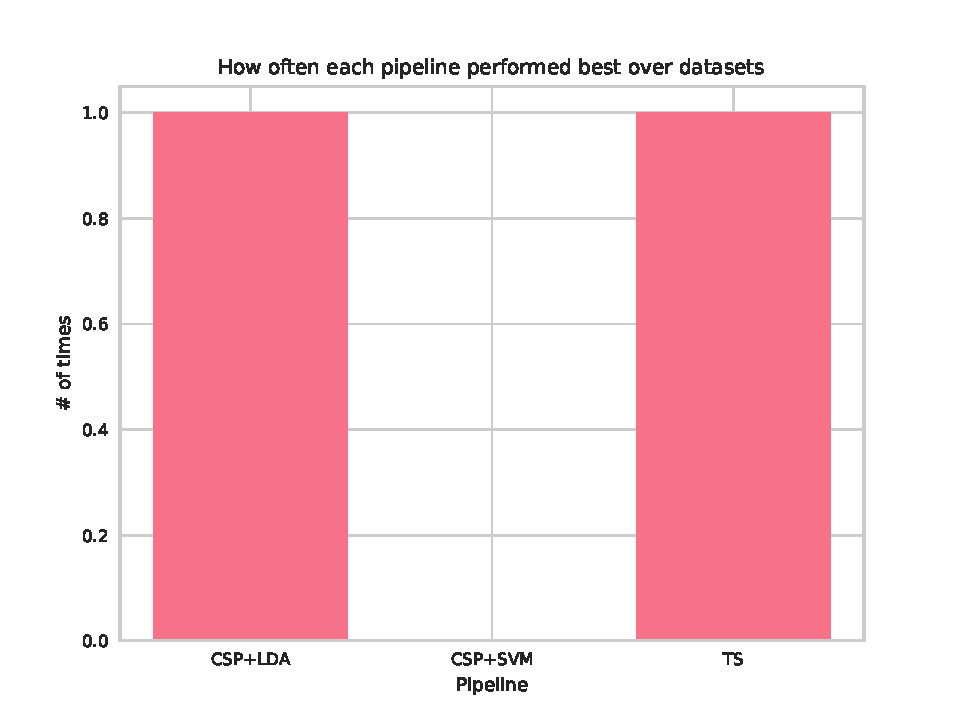
\includegraphics[width=\textwidth]{./CrossSubjectEvaluation_C3C4/summary.pdf}
    \end{subfigure}
    \caption{Cross-subject evaluation using only C3 and C4}
\end{figure*}
\begin{figure*}
    \centering
    \begin{subfigure}[t]{\textwidth}
        \centering
        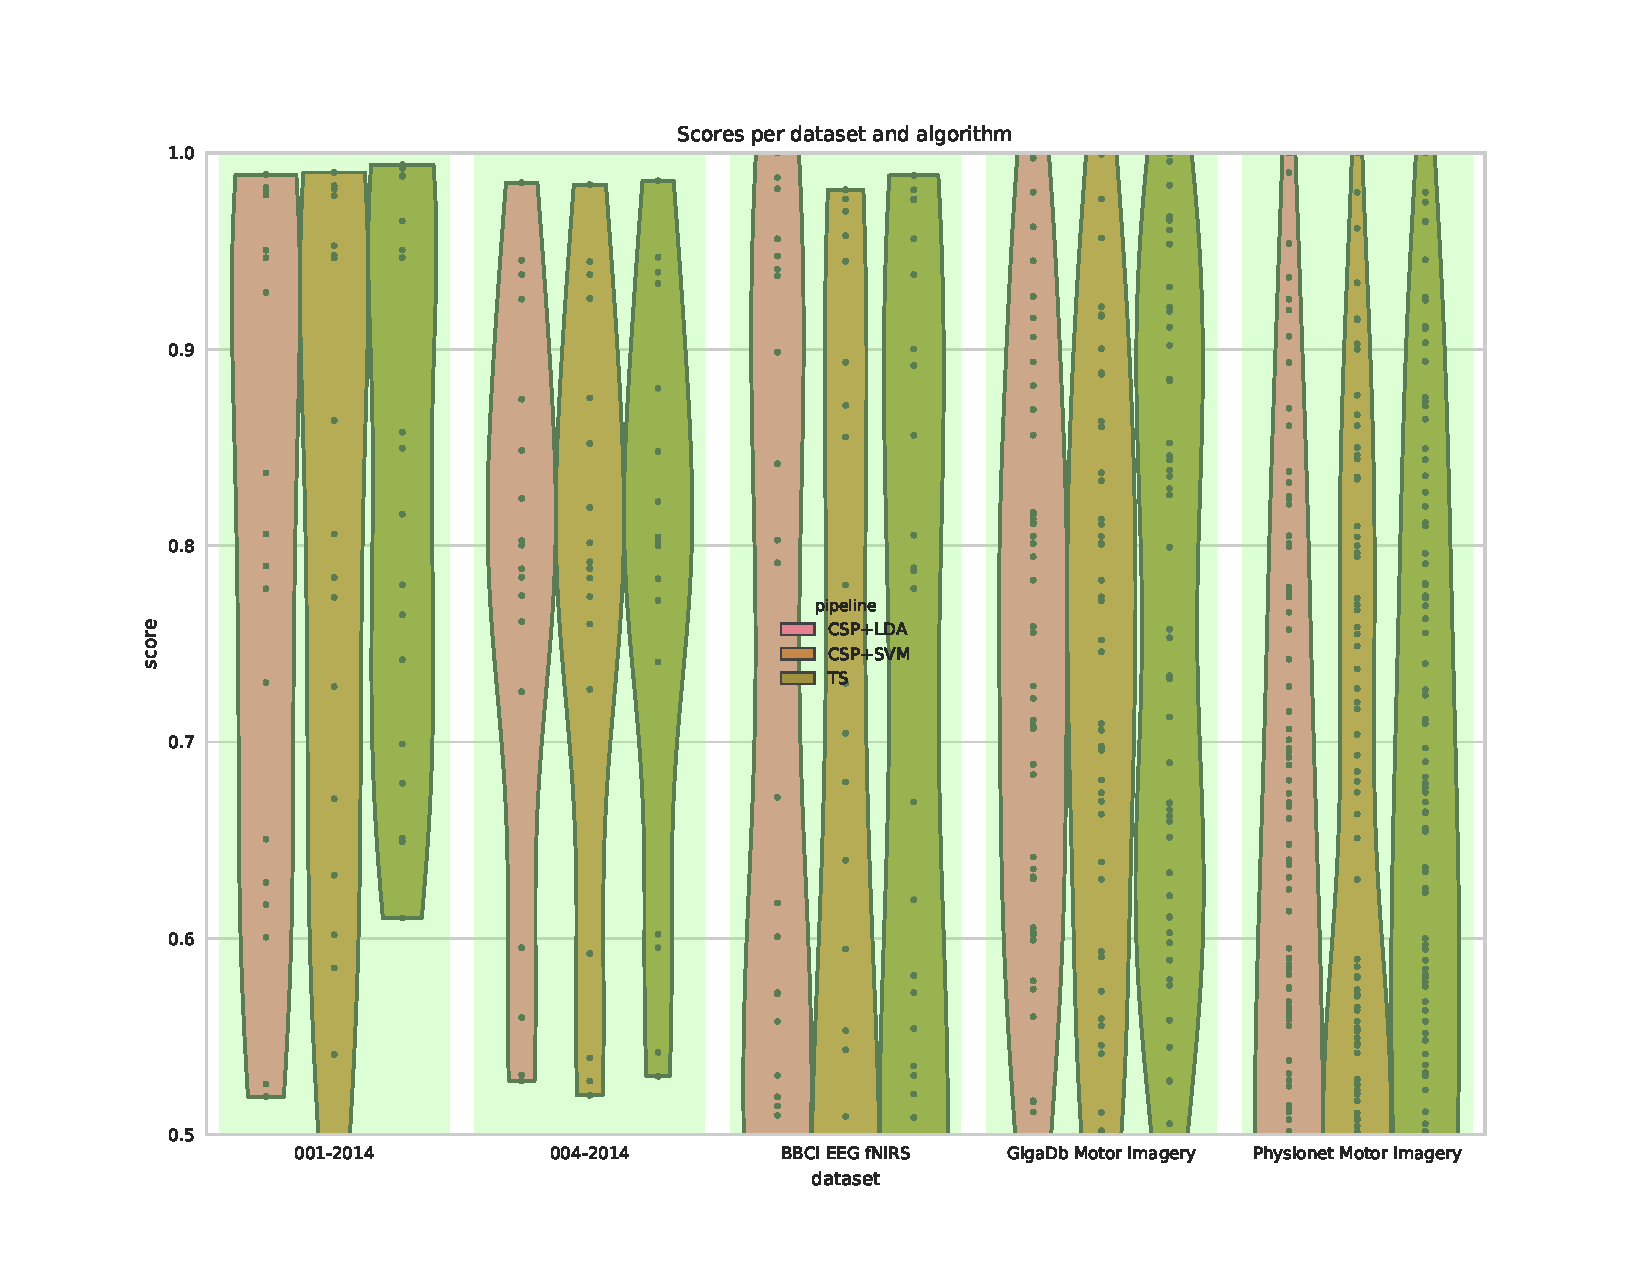
\includegraphics[width=\textwidth]{WithinSessionEvaluation_/scores.pdf}
    \end{subfigure}%
     
    \begin{subfigure}[h]{0.45\textwidth}
        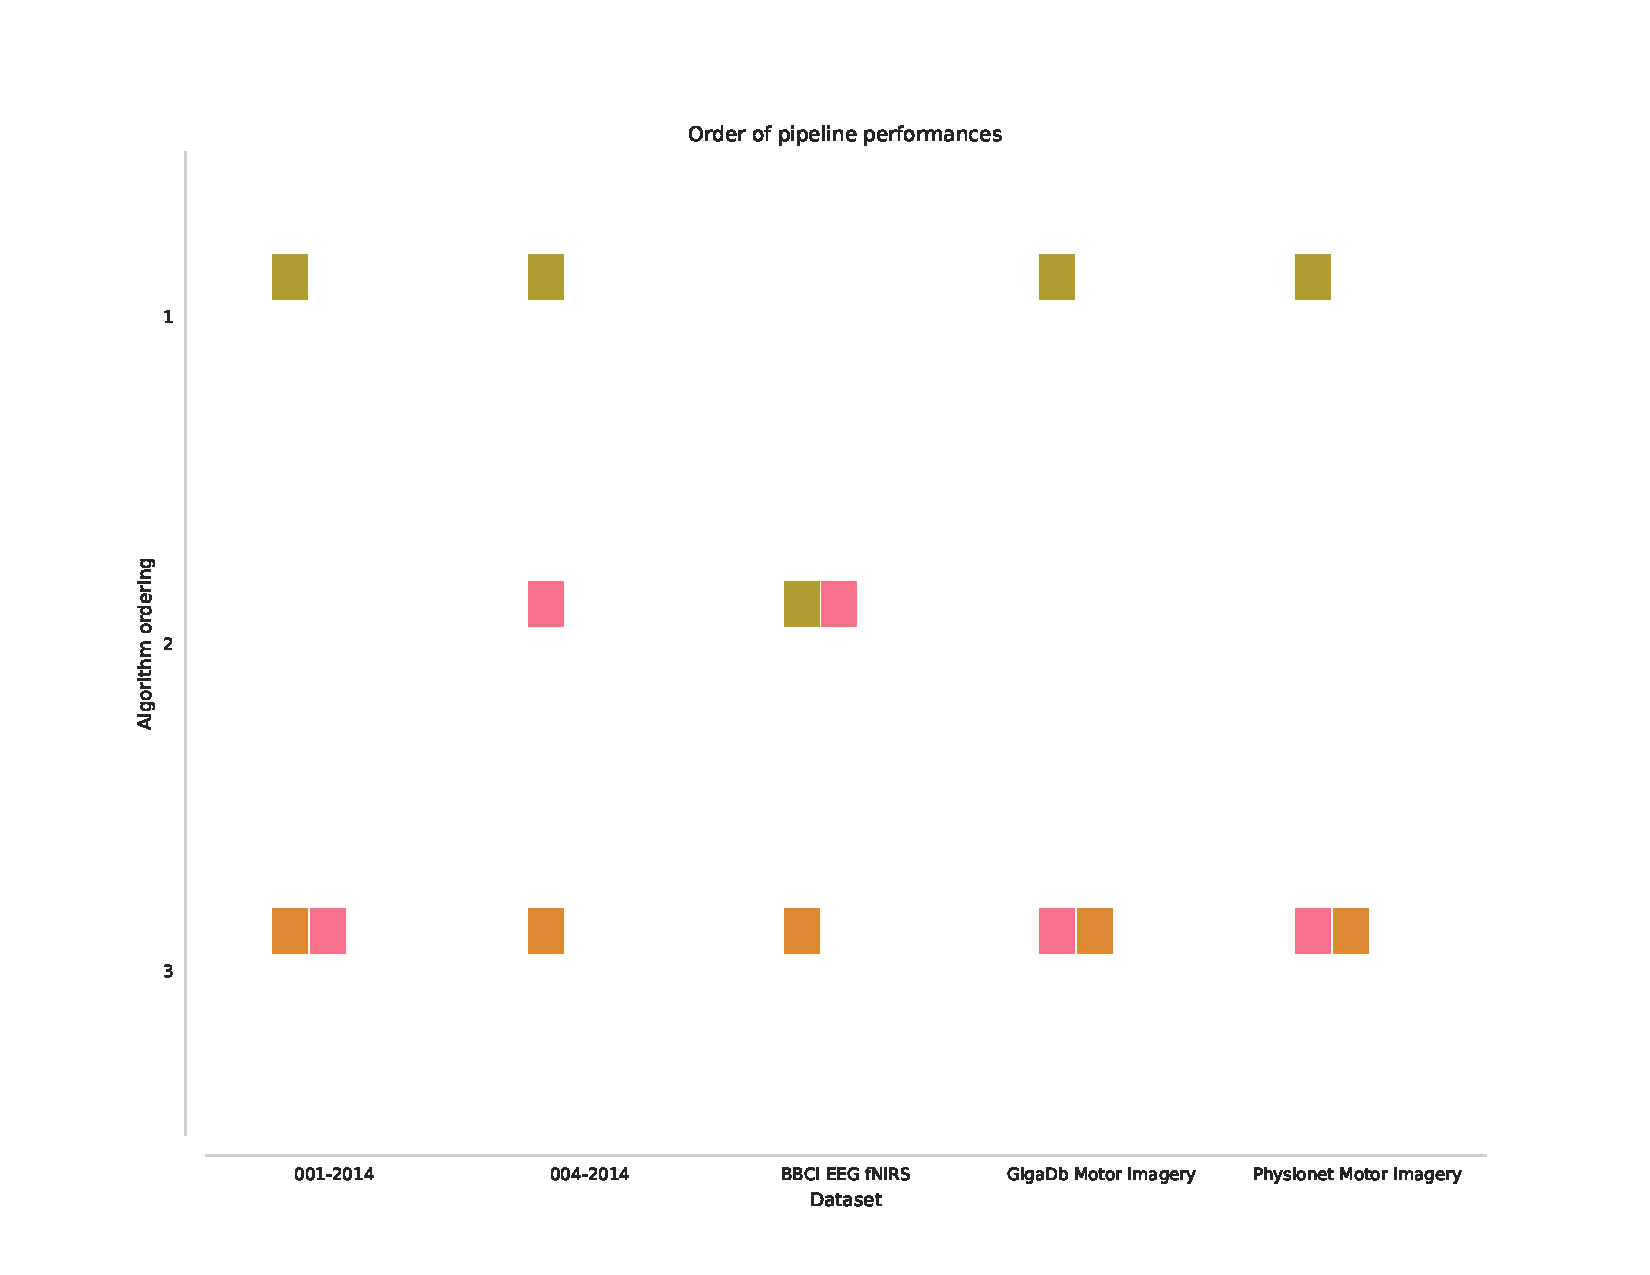
\includegraphics[width=\textwidth]{./WithinSessionEvaluation_/ordering.pdf}
    \end{subfigure}
    \begin{subfigure}[h]{0.45\textwidth}
        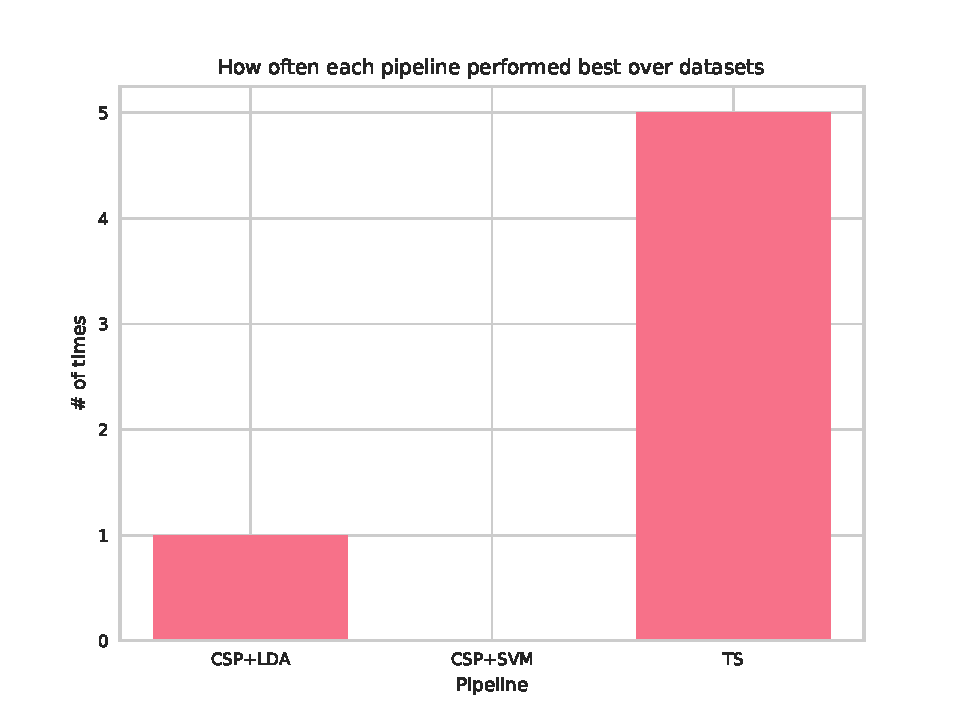
\includegraphics[width=\textwidth]{./WithinSessionEvaluation_/summary.pdf}
    \end{subfigure}
    \caption{Cross-subject evaluation using only C3 and C4}
\end{figure*}
%%% Local Variables:
%%% mode: latex
%%% TeX-master: "main"
%%% End:

\section{Discussion}
We present a system for reliably comparing BCI pipelines that is both easily
extended to incorporate new datasets and equipped with an automated statistical
procedure for determining which pipelines perform best. Furthermore, this system
defines a simple interface for submitting and validating new BCI pipelines,
which could serve to unify the many methods that exist so far. To test that
system, we present results using standard pipelines in contexts that have wide
relevance to the BCI community. By looking across multiple, large datasets, it is possible to make statements about how BCIs perform on average, without any sort of expert tuning of the processing chain, and further to see where the major pitfalls still lie.

The results of this analysis suggest that sample size and discrepancies in imagery and hardware have had a strong impact on the reproducibility of many BCI algorithms.(I'm not sure that is the main conclusion of the results) Although various regularized approaches have been validated separately to outperform the original CSP algorithm, the result here is that none of them appear to make a difference. The only algorithm that reliably out-performs the other methods is the tangent space method, but even then it is not an enormous difference. As has been known for years, the majority of variability within a BCI paradigm is not due to the algorithm, but rather the user. People who do poorly do poorly nearly regardless of the processing used on them (with some exceptions), and those that do well can often manage a simple classification task with even the simplest pipeline.


%%% Local Variables:
%%% mode: latex
%%% TeX-master: "main"
%%% End:

\section{Conclusion}
We present the MOABB project, a codebase that simplifies the application of
machine learning methods to EEG data and provides an interface to reliable,
reproducible BCI methods results. We validate the initial version of this
analysis using 275 subjects drawn from many different labs and published
open-access online, and show that with more data many previously validated
conclusions come into question.

\section*{Acknowledgements}
We would like to extend our thanks to Professor Marco Congedo for his valuable
input regarding the appropriate statistical procedure for this analysis.

\blfootnote{corresponding author: Vinay Jayaram (email: vjayaram@tue.mpg.de)}
\printbibliography
\end{document}

%%% Local Variables:
%%% mode: latex
%%% TeX-master: t
%%% End: